\documentclass[12pt]{article}
\usepackage[2120943]{easymcm}
\usepackage{mathptmx}
\usepackage{float}

\problem{A}
\title{Analysis and Prediction of Fungi Decomposition Process}

\begin{document}

	\begin{abstract}
		As an indespensable part of our terrestrial ecosystem, fungi free the carbon and other elements out from remains and debris and drive them into the cycle of ecosystem. Fungi tend to live in warm and humid environment,and are sensitive to the smallest changes.In this study, we focus on the interaction between different population of fungi and how they interact with microenvironment around them on woddy fibres. 

		In our first model, we use cmpetitive Lotka-Voterra model to demostrate the competition among different types of fungi. After the estimation of some important parameters, we simulate the gorwth of several population of  fungi  fed on infinite nutrition with no competition. The result shows that.
		
		In our second model, we mainly sudy the comprtition behavior of the fungi when woody fibres are not infinite. We add the influence of model to demonstrate the competition the competition among different types of fungi.addada. \\
		\vspace{5pt}
		\textbf{Keywords}:
	\end{abstract}
	
	\maketitle
	\tableofcontents
	\section{Introduction}
	\subsection{Problem Background}
	As an indespensable part of our terrestrial ecosystem, fungi free the carbon and other elements out from remains and debris and drive them into the ecosystem. Fungi tend to live in warm and humid environment,and are sensitive with the smallest changes.

	In this study, we focus on the interaction between different population of fungi and how they interact with microenvironment around them on woddy fibres. We use cmpetitive Lotka-Voterra model to demostrate the competition among different types of fungi.
	\subsection{Restatement of the Problem}
	Restatement
	\subsection{Our Work}
	Our work mainly includes the following:
	\begin{enumerate}[\bfseries 1.]
		\item We use Lotka-Volterra Equations to build a model to demonstrate the competition among different types of fungi.
		\item We build a model to explain how the process of decomposition is affected by temperature, moisture, and distribution of different tuypes of fungi.
		\item We analyse the sensitivity and robustness of the models above.
	\end{enumerate}
	
	\section{Model Preperation}
	\subsection{Assumptions}
	\begin{enumerate}[\bfseries 1.]
    	\item Fungi strains grow in a stable density;
	    \item Fungi grow in a 2-D plane;
    	\item The rate of decomposition of woody fibres is propotional to the number of fungi on it.
	\end{enumerate}
	\subsection{Notations}
	Important notations used in this paper are listed in Table \ref{tb:notation}
	\begin{table}[!htbp]
		\begin{center}
		\caption{Notations}
		\begin{tabular}{ccc}%两个A换行
			\toprule
			Symbol& Definition &Unit\\
			\midrule
			$T$&Temperature in Celcius&$^{\circ}C$\\
			\specialrule{0em}{1pt}{1pt}
			$M$&Moisture&MPa\\  
			\specialrule{0em}{1pt}{1pt}
			$n_i$&Fungi's Competitive Rank&$n \text{ is scaled to } [0,1]$\\
			\specialrule{0em}{1pt}{1pt}
			$\rho_{\text{hyphae}}$&Hyphae Density&$\mu g/cm^2$\\
			\specialrule{0em}{1pt}{1pt}
			$S_i$ &Popluation Size& Population of Fungi\\
			\specialrule{0em}{1pt}{1pt}
			$v_{\text{decomposition}}$ &Decomposition Rate& \% Dry weight loss  in 122 days\\ 
			\specialrule{0em}{1pt}{1pt}
			$K_i$ & Bioligical Capacity& $\mu g$\\
			\specialrule{0em}{1pt}{1pt}
			$M_{\text{woody}}$ & Weight of the Woody&$g$\\
			\bottomrule
		\end{tabular}\label{tb:notation}
		\end{center}
	\end{table}		
	\subsection{Data Collection}
	The data we use mainly include several kinds of fungi's growth rate with temperature and moisture. The data sources are summarized in Table \ref{tb:data}.
	\begin{table}[!htbp]
	\begin{center}
		\caption{Data Sources}
		\begin{tabular}{cll}
			\toprule
			\multicolumn{1}{m{5cm}}{\centering Data}
			&\multicolumn{1}{m{5cm}}{\centering Source}\\
			\midrule
			
			$\text{Different fungi trait}$& github.com/dsmaynard/\\
			$\text{Different fungi growth rate}$& github.com/dsmaynard/\\
			
			\bottomrule
		\end{tabular}\label{tb:data}
	\end{center}	
	\end{table}
	\section{Model 1:Fungi Population Prediction Model}
		\subsection{Competitive Lotca-Voterra Equations}
        We assume that there is only one kind of fungi, Phlebia acerina DR60 A8A,and using data as follows:
\begin{align}%单位改正体,下同
    T=22^{\circ}C,M=-0.5\text{MPa},n=0.97,v_{\text{ex}}=8.51\text{mm/day},\nonumber\\
    \rho_{hy}=0.27\mu g/cm^2,v_{de}=73.39\pm 10.22\%/122\text{days}\nonumber
\end{align}



where r is pamrameter of describing the speed of growth, and k is bioligical capacity.

We assume that there are N kinds of different fungi, and the biomass of each kind of fungi is $S_i$. We only concern about the relative biomass of each kind of fungi, so we substitute $S_i$ with $x_i=S_i/K_i$.

We use the Competitive Lotca-Voterre equations, a model for the population dynamics of species competing for some resource. 

\begin{align}
    \frac{dS_i}{dt}=r_i S_i  (1- \frac{\sum_{j=1}^{N}\alpha_{ij}S_j}{K_i})
\end{align}

Using the substitution $x_i=S_i/K_i$, the equations can be written as below:

\begin{align}
    \frac{dx_i}{dt}=r_i x_i  (1- \frac{\sum_{j=1}^{N}\alpha_{ij}x_jK_j}{K_i})
\end{align}

where
\begin{align}
    r_i&=\frac{v_{extension}}{R}\\
    K_i&=C\rho_i,C=const\\
    \alpha_{ij}&=\exp{1-\frac{n_i}{n_j}}\\
    \epsilon&=0.33
\end{align}

$\epsilon\:$is efficiency, according to the reference[3].
		\subsection{Parameter Estimation of LV Equations}
        We assume that $\alpha_{ij}=\exp(1-n_i/n_j)$, making the fungi with larger n having advantages over fungi with smaller n.
			\subsubsection{Carrying Capacity:K}
			\subsubsection{Inherent Per-capita Growth Rate:r}
            When there's only one kind of fungi, it evolve as he equation below:

            \begin{align}
                \frac{dx(t)}{dt}=r(T,M)x(t)(1-\frac{S(t)}{K(T,M)})
            \end{align}
            So we assume that $r=\left< \frac{dS}{dt} \right>$
		\subsection{Results}
        We choose several kinds of fungi, the data are shown as follow:

and the result after enough long time of evolution is shown in Figure 1, where temperature $T=25^{\circ}C$, moisture $M=-0.5MPa$

\begin{figure}[H]
    \centering
    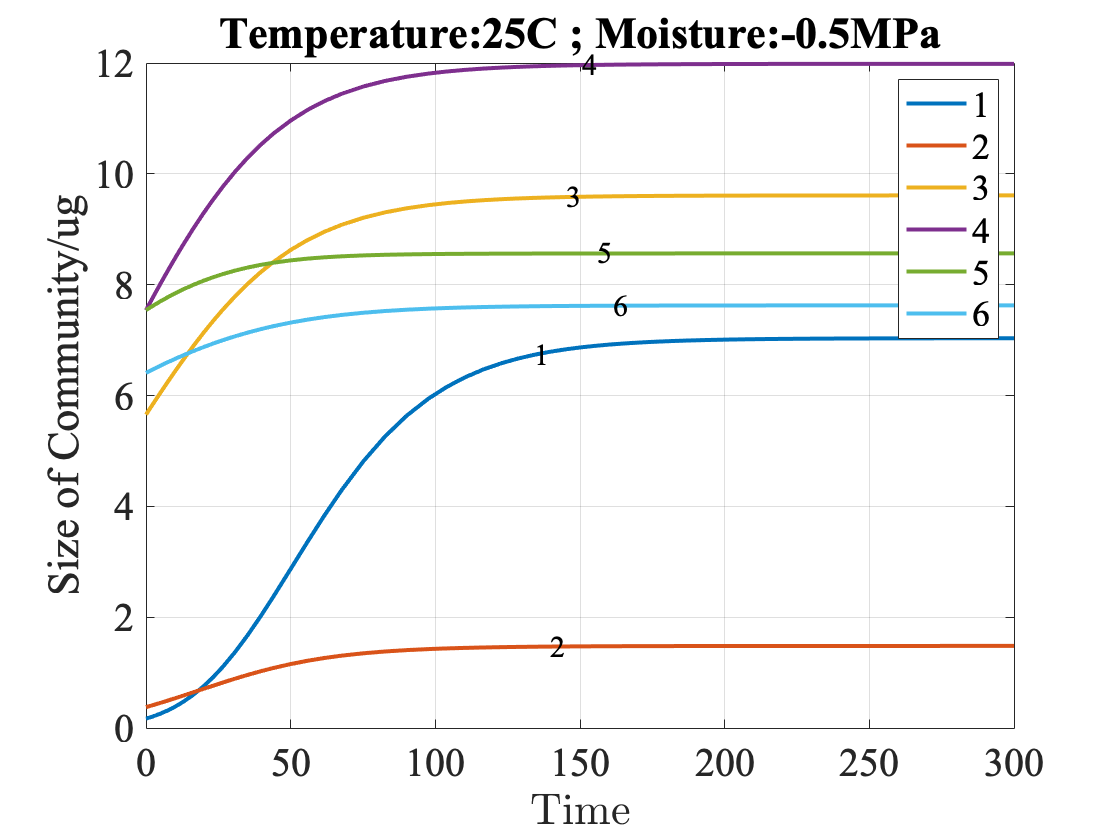
\includegraphics[width=.6\textwidth]{25_05.png}
    \caption{The result of Model 1}\label{fig:result1}%引用标记
    \end{figure}

%---------------------------------------------			
	\subsection{Detail 1 about Model 1}

%-------------------------------------------------








	\section{Model 2:Woody Fibres Decomposition Model}
	\subsection{Decomposition Equations}
	\subsection{Single Population}
		\subsubsection{Population Equation}
		According to the reference[3], the decomposition of wood confirms to the following model:

\begin{align}
    \frac{dS}{dt}=rS(1-S/K)\times M_{woody}\\
    \frac{dM_{woody}}{dt}=-\frac{r}{\epsilon}SM_{woody}
\end{align}
		\subsubsection{Results}
	\subsection{Multi Population}
		\subsubsection{Population Equation}
		\subsubsection{Results}
	

We assume that there are N kinds of different fungi, and the biomass of each kind of fungi is $S_i$. We only concern about the relative biomass o feach kind of fungi, so we substitute $S_i$ with $x_i=S_i/K_i$.

We use hte Competitive Lotca-Voterre equations, a model for the population dynamics of species competing for some resource. 

\begin{align}
    \frac{dS_i}{dt}=r_i S_i  (1- \frac{\sum_{j=1}^{N}\alpha_{ij}S_j}{K_i})
\end{align}
Using the substitution $x_i=S_i/K_i$, the equations are shown as below:
\begin{align}
    \frac{dx_i}{dt}=r_i x_i  (1- \frac{\sum_{j=1}^{N}\alpha_{ij}x_jK_j}{K_i})
\end{align}
where
\begin{align}
    r_i&=\frac{v_{extension}}{R}\\
    K_i&=C\rho_i,C=const\\
    \alpha_{ij}&=\exp{1-\frac{n_i}{n_j}}\\
    \epsilon=0.33\text{is efficiency, according to the reference[3]}
\end{align}

The results are shown in Figure \ref{fig:result}

\begin{figure}[H]
	\centering
	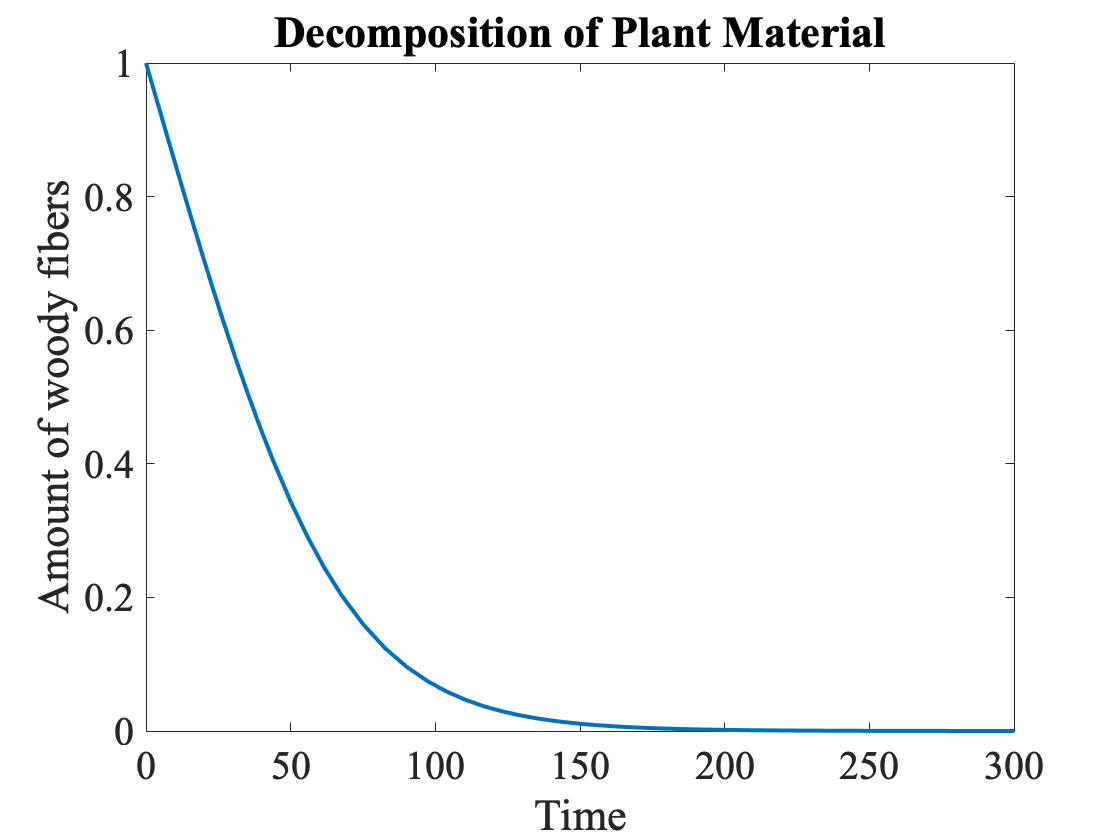
\includegraphics[width=.6\textwidth]{25_05_de.png}
	\caption{Decomposition Model}\label{fig:result}
\end{figure}

	\section{Discussion}
\subsection{Rapid Fluctuations}
\subsection{Prediction Under Different Environment}
	\section{Test the Models}
\subsection{Sensitivity Analysis}
\subsection{Robustness}
	\section{Conclusion}
\subsection{Summary of Results}
\subsection{Strength}
\subsection{Possible Improvements}
	\documentclass[12pt]{article}
\usepackage{mathptmx}
\usepackage{float}

\begin{document}
Fungi play a crucial role in the balance of  our ecosystem. They scatter in most habitats on Earth, preferring moist and temperate conditions, and are very seneitive of that. Fungi are one of the major decomposers of nature, thanks to their versatile metabolism, fungi break down organic matter, which would not otherwise be recycled.

Fungi are important to our daily life. Fungi are important decomposers in most ecosystems. They free the carbon in the debris remains and waste of living creatures, and drive then back into the carbon cycle.
If fungi and bacteria did not return them to the environment via their metabolism, it would remain tied up in rotting organic matter.

Our recent study shows that fungi    decomposites 75\% of woody fibres they live on in just * days, and the process are extermely sensitive to the temperature, moisture and the pressure other fungi gives to them. 

According to the research, the change of climate will always lead to the change of fungi living there. if123 
\end{document}
	\section{Referencese}
\begin{thebibliography}{99}

    \bibitem{2}Dang, Christian K. , et al. "Temperature oscillation coupled with fungal community shifts can modulate warming effects on litter decomposition." \emph{Ecology} 90.1(2009).
\end{thebibliography}
\end{document}